%Autor: Prof. Me. Phyllipe Lima
%Contato: phyllipe_slf@yahoo.com.br
%Modelo para escrita de artigos científicos para o curso de Pós-Graduação em Desenvolvimento de Aplicações para Dispositivos Móveis e Cloud Computing do INATEL - Instituto Nacional de Telecomunicações. Este template LaTeX é uma adaptação do modelo doc desenvolvido pelos professores Carlos Ynoguti e Dayan Guimarães
\documentclass[11pt,twocolumn]{article} 
%para Español {BEGIN}
 
% La sigientes lineas son para podel escribir en español usando el
%teclaso y poder usar el corrector de idioma automático. 
%OJOJOJOJOJOJOJOJOJOJOJOJOJO:  
%También es necesario el spanish como opción de la clase.
%OJOJOJOJOJOJOJOJOJOJOJOJOJO:  
\usepackage[spanish]{babel}
\selectlanguage{spanish}
\spanishdecimal{.}
\usepackage[utf8]{inputenc}
%para Español {END}

%Use esse arquivo para incluir novos pacotes

\usepackage[
top=0cm,
bottom=1.78cm,
left=1.65cm,
right=1.65cm,
headheight=2.9cm,
headsep=0cm,
includehead
%showframe
]{geometry}
%\usepackage[justification=centering]{caption}
\usepackage{inatelPOS}
\usepackage{times}
\usepackage{graphicx}
\usepackage{url,hyperref}
\usepackage[utf8]{inputenc}
\usepackage{float}
\usepackage{caption}
\usepackage{mathtools}
\usepackage[hang,flushmargin]{footmisc} 
\usepackage{xcolor}
\usepackage{wrapfig} %usado para envolver figura com texto
%\usepackage[portuguese]{babel}
\usepackage{fancyhdr}
\usepackage{etoolbox}
\usepackage{adjustbox}
\usepackage{comment}
\usepackage{relsize} %usado por comandos \mathlarger
%\usepackage{mathptmx}

\begin{document}

%Ajustes na figura
\captionsetup[figure]{labelformat={default},labelsep=period,font=footnotesize, name=\footnotesize{Fig.},justification=raggedright,singlelinecheck=false}
%\pagenumbering{gobble}

%Ajustes na tabela
\captionsetup[table]{labelformat={default},labelsep=newline,font={sc,footnotesize},name=\footnotesize{TABELA}}
\renewcommand{\headrulewidth}{0pt}

\pagestyle{fancyplain}{%
    \fancyhf{} % limpa os campos
    \chead{ \textcolor{black!50}{\textbf{
    UNIVERSIDAD DE SONORA\\ 
    Licenciatura en Física para la clase de 
    Física Computacional \\
    27 de enero de 2019\\
    Grupo 3
    }}}
    \cfoot{\thepage}
}

\AtBeginEnvironment{tabular}{\footnotesize}
\title{\Huge \bf Combatiendo el Calentamiento Global}

\author{\large 
Castillo Espinoza Aarón Sebastián}
\maketitle

\section{Introducción}
El propósito de este trabajo es hacer una reflexión acerca del calentamiento global, las consecuencias que este ha traído hasta el momento y lo que pasara en un futuro no muy lejano si no cambiamos nuestra forma de vivir el día a día. Hoy en día nos encontramos a una temperatura de $1^\circ$C mayor a la era preindustrial y se estima que esta aumenta a razón de $0.2^\circ$C cada 10 años

El pasado 6 de Octubre se presento Reporte del Panel Intergubernamental de Cambio Climático (IPCC) en el cual resaltan la importancia de reducir a la mitad nuestras emisiones de $CO_2$ en los próximos 10 si queremos salvar el planeta. En este reporte se hace énfasis de que el limite que existe para el aumento de temperatura es de $1.5^\circ$C aunque el escenario planteado no es nada amigable con esa temperatura, es mucho mejor y más prometedor que llegar a $2^\circ$C. Si bien $0.5^\circ$C no parece mucho, cuando hablamos de un aumento permanente a nivel mundial significará consecuencias enormes no solo a los ecosistemas naturales, si no también a la economía humana. \textcolor{blue}{"Limitar el calentamiento global a $1.5^\circ$C en comparación con $2^\circ$C reduciría los impactos desafiantes sobre los ecosistemas, la salud humana y el bienestar}, dijo Priyardarshi Shukla, Presidente del Centro Mundial para el Medio Ambiente y la Energía de la Universidad de Ahmedabad en la India y Autor del Informe Especial.

El secretario general de la ONU, Antonio Guterres emitió un comunicado en el que dijo que alcanzar esta meta requiere \textcolor{blue}{"una acción urgente y mucho más ambiciosa para reducir las emisiones a la mitad para 2030, y alcanzar las emisiones netas cero para 2050}.

\begin{figure}[H]
  \centering 
  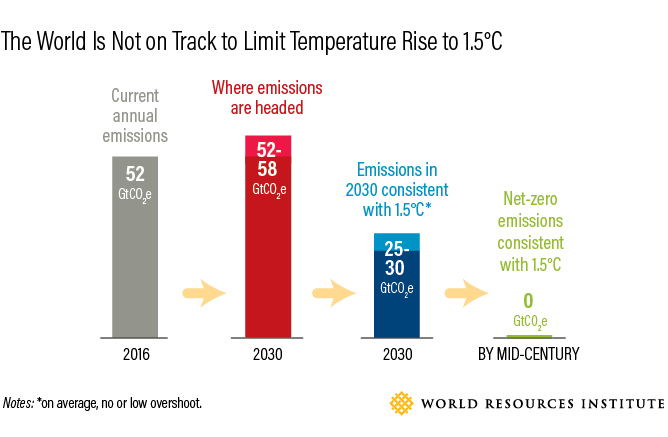
\includegraphics[width=0.32\textwidth]{figuras/grafica.png}
  \caption{Imagen de World Resources Institute}
  \label{fig:revista_inatel}
\end{figure}




\section{Puntos Importantes}
A continuación presento algunos de los puntos más importantes que presentaron durante el reporte del IPCC: 


\subsection{\textcolor{red}{La importancia de medio grado}}
Este medio grado de medio grado es la diferencia que hay entre la vida y la muerte para muchas especies animales, así como la supervivencia de importantes ecosistemas marinos como lo es el coral, siendo este el hogar de muchas especies pequeñas que se encuentran al principio de la cadena alimenticia. Se estima que si la temperatura llega a los $2^\circ$C se perderán el 99\% de estos, mientras que si la temperatura solo alcanza los $1.5^\circ$C solo se perderían del 70 al 90\%. \textcolor{blue}{"Limitar el calentamiento global a $1.5^\circ$C en comparación con $2^\circ$C reduciría los impactos desafiantes sobre los ecosistemas, la salud humana y el bienestar, facilitando el logro de los Objetivos de Desarrollo Sostenible (ODS) de las Naciones Unidas}, dijo Priyardarshi Shukla, Co-presidente del Grupo de Trabajo III del IPCC.

\subsection{\textcolor{red}{Es posible, debemos movernos rápido}}
\textcolor{blue}{"Limitar el calentamiento a $1.5^\circ$C es posible dentro de las leyes de química y física, pero hacerlo requeriría cambios sin precedentes}, dijo Jim Skea, Co-presidente del Grupo de trabajo III del IPCC. Se recalca la necesidad de reducir las emisiones de $CO_2$ en al menos un 45\% para el 2030 con respecto a las de 2010 y continuar con los esfuerzos para alcanzar cero emisiones para 2050. Para lograr esto el informe nos exhorta a hacer grandes cambios en el uso de la tierra y la generación de energía para la industria, transportes y edificios en todas las ciudades del mundo. Es un desafío enorme el de mantenernos por debajo $2^\circ$C, ya que requiere que la infraestructura de combustibles fósiles se elimine gradualmente y que se elimine carbono a gran escala de la atmósfera, dice Glen Peters , Director de Investigación en el Centro de Investigación Climática Internacional de Noruega. \textcolor{blue}{"Mantenerse por debajo de 1.5 C simplemente requiere que la transformación sea más rápida y más profunda que para $2^\circ$C}, dijo Peters.

\subsection{\textcolor{red}{Soluciones Presentadas}}
En el reporte del IPCC se establecen varias soluciones para lograr la meta de $1.5^\circ$C, sin embargo, todas requieren  
esfuerzos sin precedentes para reducir la quema de combustibles fósiles en menos de 10 años y que estos lleguen a 0 en 30 años. Es decir, para medio siglo debemos lograr que ningún hogar, negocio o edificio debe calentarse a base de gas o petroleo, no más vehículos alimentados por Diesel o gasolina y aquellas industrias de producción pesada debe utilizar fuentes de energía limpia o bien, almacenar sus emociones de $CO_2$ permanentemente. Esto significara un gasto enorme de capital por parte de las empresas para apegarse al plan de reducción o un paro total de sus actividades lo que implicaría que estas cierren sus puertas como es el caso de centrales eléctricas y de gas.
\begin{figure}[H]
  \centering 
  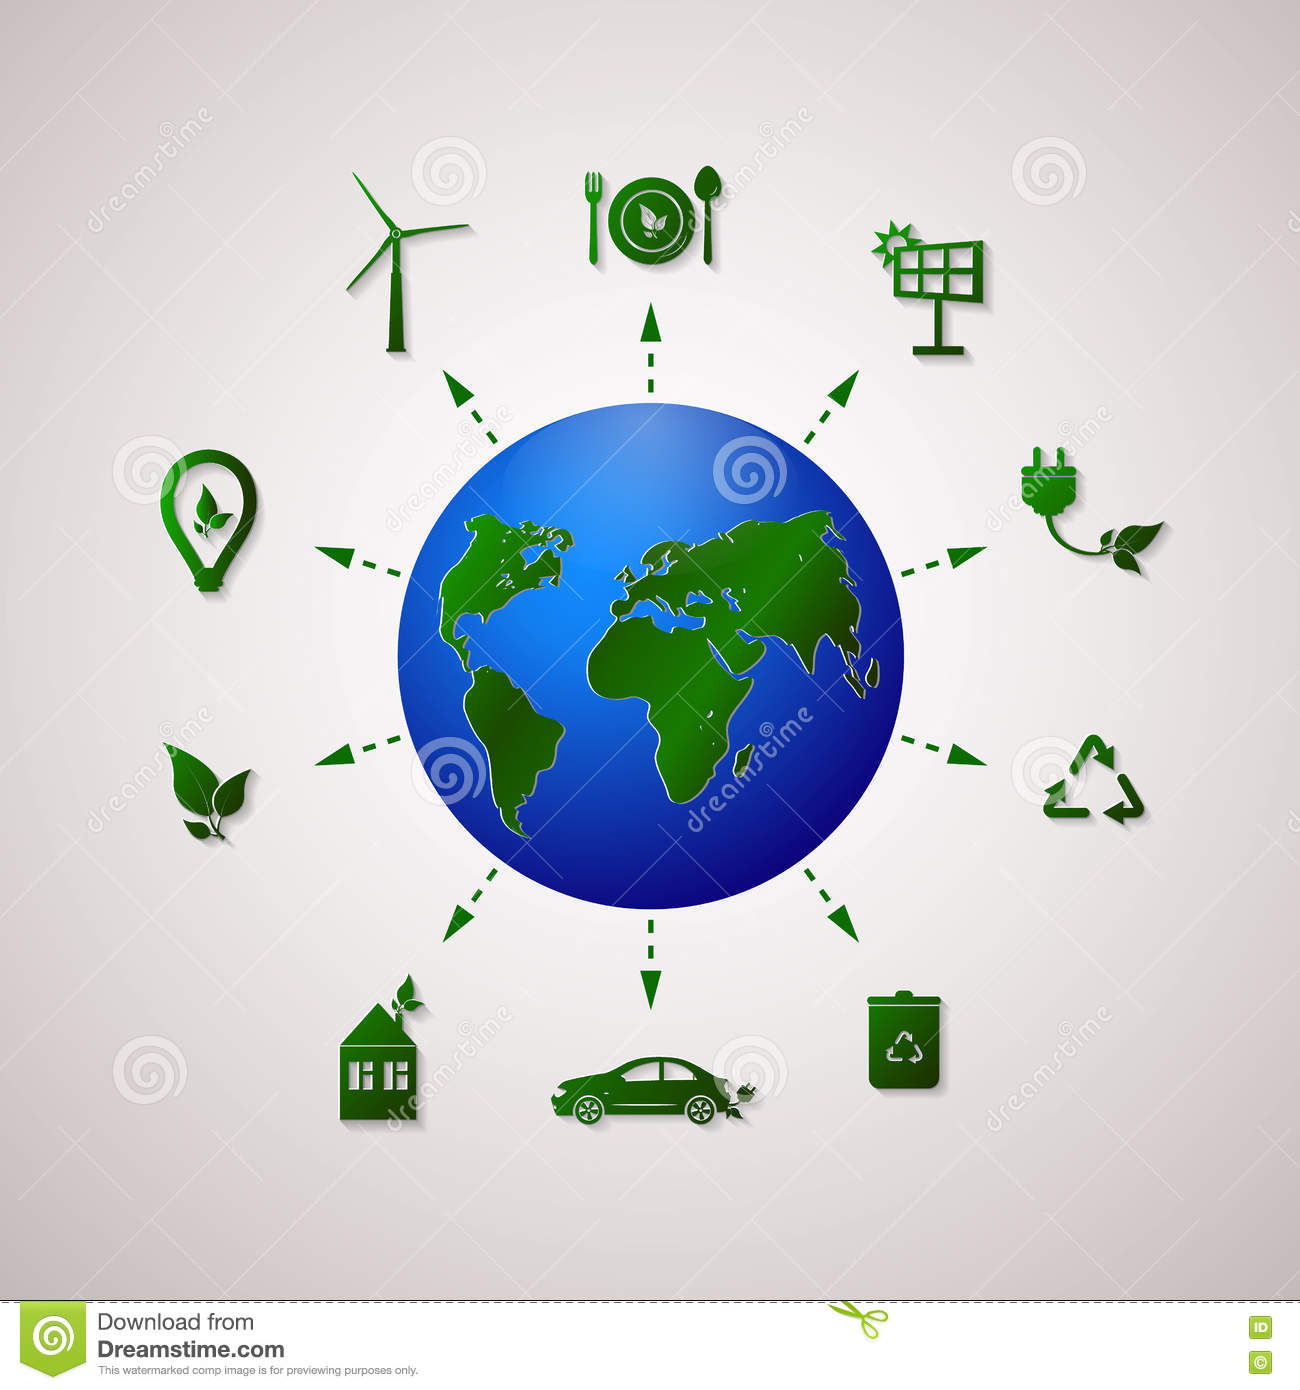
\includegraphics[width=0.15\textwidth]{figuras/planeta.jpg}
  \caption{Imagen de Dreamstime.com}
  \label{fig:revista_inatel}
\end{figure}

\subsection{\textcolor{red}{Reforestación y áreas verdes}}
En el reporte que se requiere de 1 a 7 millones de $Km^2$ de tierras convertidas en cultivos de bioenergía y hasta 10 millones de $Km^2$ más de bosques para el 2050. Para Deborah Lawrence , experta en bosques de la Universidad de Virginia, los bosques desempeñan un papel muy mucho mas importante en la reducción de las emisiones, pues según ella \textcolor{blue}{"Los bosques brindan un servicio súper importante para la humanidad al eliminar actualmente un 25\% del $CO_2$ de la atmósfera}. la reforestación representa un 18\% de las reducciones necesarias para el año 2030 dice Lawrence, países como Brasil, China, India, México, Australia, Estados Unidos, Rusia y la Unión Europea se están sumando a la reforestación. Proteger e incrementar los bosques tropicales es especialmente importante ya que enfrían el aire y son clave para crear precipitaciones regionales para el cultivo de alimentos.



\section{Reflexión}
A lo largo de la elaboración de este trabajo me di cuenta de que todo lo que hacemos, incluso respirar, genera una gran cantidad de $CO_2$ para la cual no hay forma de contener o reducir. A diferencia de lo que muchos creen, incluyendo al presidente de los Estados Unidos Donald Trump, el calentamiento global no es ningún mito; se trata de una realidad a la cual hay que enfrentarnos ya si queremos tener un futuro, no es posible que confiemos en películas y libros de ciencia ficción que "predicen" el fin del mundo y no creamos en lo que la ciencia nos dice acerca de este.
Las soluciones están planteadas, depende de nosotros implementarlas o no, si queremos seguir viviendo en este planeta o no. 
Hoy en día existen muchos proyectos que pueden ayudar en gran medida a nuestro planeta como lo son las torres eólicas, los paneles solares, las plantas hidroeléctricas, la obtención de petroleo a partir de basura, un proyecto mexicano, que obtiene petroleo sin la generación de $CO_2$. Otro proyecto mexicano es la torre que absorbe $CO_2$ y genera oxigeno mediante la utilización de alga viva. En Asia existe el proyecto de una torre que limpia el aire de $CO_2$, regresando aire limpio al ambiente mientras que el carbono que obtiene lo comprime y genera diamantes de este, los cuales son vendidos para la construcción de mas torres como esta. Todos y cada un de estos proyectos son una gran opción para limpiar nuestro ambiente, sin embargo la tecnología que se emplea en estos proyectos aun es muy costosa para su producción en masa aparte de que genera una gran disminución de ganancias para la industria petrolera y energética.

Yo creo que hoy ya no es momento de estar pensando en obtener ganancias grandes ni ser el numero uno en ventas alrededor del mundo, si no que debemos buscar la manera de mejorar nuestro ambiente e intentar salvar nuestro planeta, el tiempo esta corriendo y es muy limitado


\section{Referencias Bibliográficas}
National Graographic, "Impacto del cambio climático peor de lo esperado, advierte informe global":
\textcolor{blue}{https://www.nationalgeographic.com/environment/2018/10/ipcc-report-climate-change-impacts-forests-emissions/}

Noticias de la ONU, "Un informe sobre el calentamiento global, una 'llamada de atención' para advertir al jefe de la ONU":
\textcolor{blue}{https://news.un.org/en/story/2018/10/1022492}

World Resources Institue, "8 Things You Need to Know About the IPCC $1.5^\circ$C Report":
\textcolor{blue}{https://www.wri.org/blog/2018/10/8-things-you-need-know-about-ipcc-15-c-report}




 

\end{document}

